\documentclass{article}
\usepackage{C:/Users/guitr/Documents/git_repositories/tpack/tpack}
% \usepackage{C:/Users/Admin-PC/Documents/git_repository/tpack/tpack}
% \usepackage{/home/tr0fin0/git_repositories/tpack/tpack}


\title{MI201 - Apprentissage Automatique}
\project{Résumé Théorique - Decision Tree}
\author{Guilherme Nunes Trofino}
\authorRA{2022-2024}


\makeatletter
\begin{document}\selectlanguage{french}
\maketitle
\setlength{\parindent}{0pt}

\newpage\tableofcontents

\section{Introduction}
\subfile{C:/Users/guitr/Documents/git_repositories/classes_ensta/intro.tex}
% \subfile{C:/Users/Admin-PC/Documents/git_repository/classes_ensta/intro.tex}
% \subfile{/home/tr0fin0/git_repositories/classes_ensta/intro.tex}

\section{Apprentissage}
\subsection{Algorithme}
On considère que l'algorithme peut être définie par la définition suivante:
\begin{definition}
    % Un arbre de décision est un modèle composé d'une collection de "questions" organisées de manière hiérarchique en forme d'arbre. Les questions sont généralement appelées condition, split ou test. Nous utiliserons le terme "état" dans cette classe. Chaque nœud non feuille contient une condition, et chaque nœud feuille contient une prédiction.
    % \paragraph{Répresentation}Les arbres botaniques poussent généralement avec la racine en bas. Toutefois, les arbres de décision sont généralement représentés par la racine, le premier nœud, en haut.
    % \paragraph{Surapprentissage}In general, the deeper you allow your tree to grow, the more complex your model will become because you will have more splits and it captures more information about the data and this is one of the root causes of overfitting in decision trees because your model will fit perfectly for the training data and will not be able to generalize well on test set.
    Prédiction a partir de différents questions aux attributs des données en les divisant à chaque décision. On considère la nomenclature:
    \begin{figure}[H]
        \centering
        \begin{forest} % from https://tex.stackexchange.com/a/304002/121799
            for tree={
                s sep = 10mm,   % Horizontal Distance
                l = 0mm,        % Vertical Distance
                where n children={0}{ev}{iv},
                l+=8mm,
                if n=1{
                    edge label={
                        node [midway, left] {1}
                    }
                }{
                    edge label={
                        node [midway, right] {0}
                    }
                }
            }
            [?
                [?
                    [0.3] [0.3]
                ]
                [?
                    [0.2]
                    [?
                        [0.1] [0.1]
                    ]
                ]
            ]
        \end{forest}
        \caption{Representation Arbre de Décision}
    \end{figure}
    On considère:
    \begin{enumerate}[noitemsep]
        \item \textbf{node}:
        \begin{enumerate}[noitemsep]
            \item \texttt{root}: première node, représente tous les données;
            \item \texttt{decision}: sub-node qui se divide en d'autre sub-nodes en représentant une question;
            \item \texttt{leaf}: node qui ne se divide pas, présente une partie des données;
        \end{enumerate}
        \item \textbf{splitting}: process division d'une node en sub-nodes;
        \item \textbf{pruning}: process d'enlever une node;
    \end{enumerate}
    On considère pour convention:
    \begin{enumerate}[noitemsep]
        \item \textbf{gauche} représente réponse \texttt{true}, ou 1;
        \item \textbf{droite} représente réponse \texttt{false}, ou 0;
    \end{enumerate}
    On considère que la profondeur p d'une arbre de décision est simply the largest possible length between the root to a leaf.
    \begin{remark}
        maximum depth would be N-1, where N is the number of training samples. You can derive this by considering that the least effective split would be peeling off one training example per node.
    \end{remark}
\end{definition}
\begin{remark}
    L'Arbre de Décision n'est pas trop sensible aux données mais de toute façon ont tendance d'avoir une variance élevée. 
\end{remark}
On classifiée l'Arbre de Décision en:
\begin{enumerate}[noitemsep]
    \item \textbf{Classification}: les outputs sont des categories;
    \item \textbf{Regression}: les outputs sont des numéros;
\end{enumerate}
À chaque noeud on choisit le test $T$ qui maximise le gain en homogénéité:
\begin{equation}
    T = \arg_{T}\max(Gain(D, T))
\end{equation}
Où:
\begin{enumerate}[noitemsep]
    \item $D$: population de données;
    \item $Gain(D, T)$: gain of the test T in the population D:
    \begin{equation}
        Gain(D, T) = I(D) - \sum_{i} (p(D_{i}|D, T) \cdot I(D_{i}))
        \qquad\text{où}\qquad
        p(D_{i}|D, T) = \frac{|D_{i}|}{|D|}
    \end{equation}
    Où:
    \begin{enumerate}[noitemsep]
        \item $I(D)$: Critère d'Hétérogénéité;
        \item $p(D_{i}|D, T)$: Proportion de Données dans D sélectionnées par la branche $i$;
    \end{enumerate}
\end{enumerate}
La décision sera fait à partir d'une critère arbitraire, entre les plus communs on a:
\begin{enumerate}[noitemsep]
    \item \textbf{Indice de Gini}: seulement pour une arbre binaire;
    \begin{equation}
        I(D) = \sum_{i} p_{i}(D)\cdot(1- p_{i}(D))
    \end{equation}
    \item \textbf{Indice d'Erreur};
    \begin{equation}
        I(D) = 1 - \max_{i} (p_{i}(D))
    \end{equation}
    \item \textbf{Entropie};
    \begin{equation}
        I(D) = -\sum_{i} p_{i}(D)\cdot\log_{2}(p_{i}(D))
    \end{equation}
\end{enumerate}
À la fin on aura une division des données qui peut se rassembler à le suivant:
\begin{figure}[H]
    \centering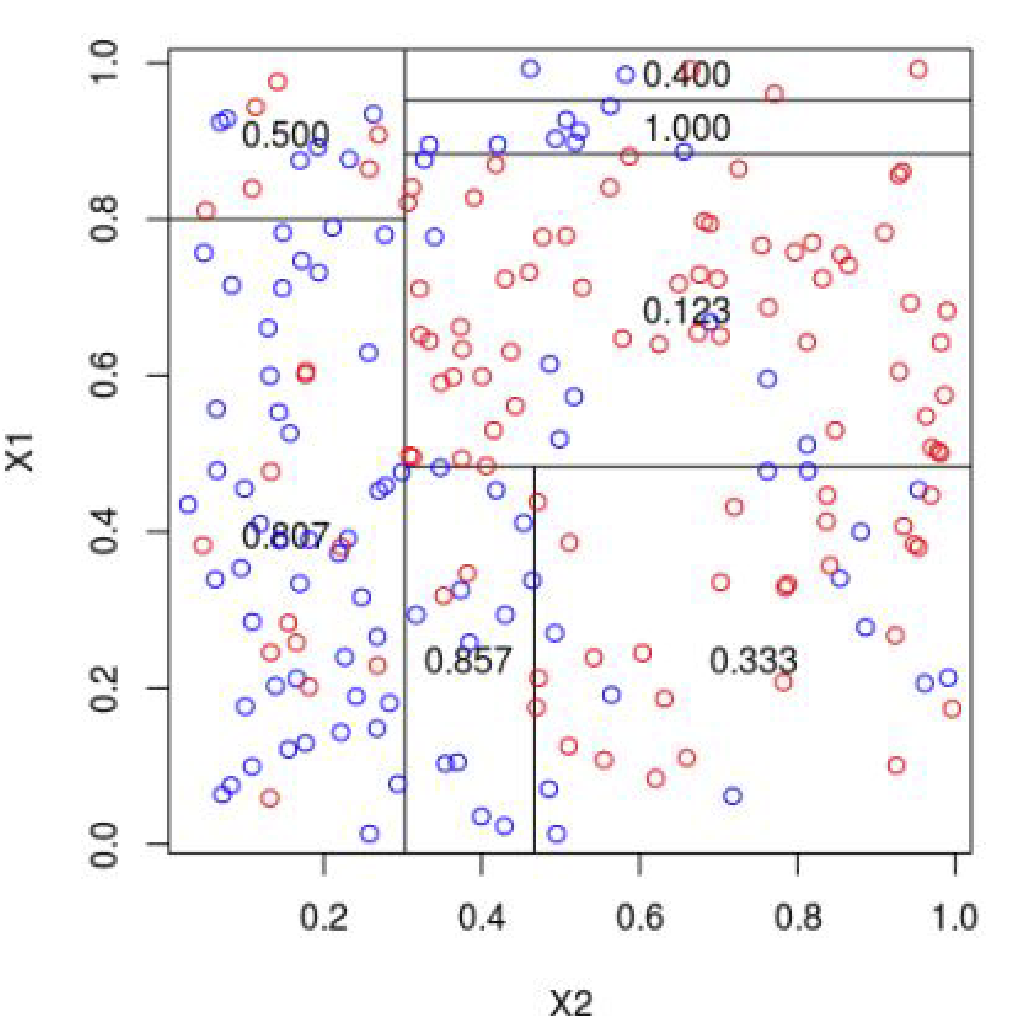
\includegraphics[height=50mm]{images/tree_diagram.png}
    \caption{Representation Division}
\end{figure}
La choix de la profondeur p de l'Arbre de Décision déterminera la qualité de la prédiction. Si on augment p la prediction améliore. Généralement on aura le comportement suivant:
\begin{table}[H]
    \centering\begin{tabular}{lll}
        p $\uparrow$   & biais $\downarrow$ & variance $\uparrow$\\
        p $\downarrow$ & biais $\uparrow  $ & variance $\downarrow$\\
    \end{tabular}
    \caption{Comportement Decision Tree}
\end{table}
Comme les Arbres de Décision ont une tendance au surapprentissage on peut utiliser des \textbf{Forêts Aléatoires}:
\begin{definition}
    Construction de plusieurs arbres se basant non seulement sur des échantillons différents mais aussi sur des variables différents. On considère le diagramme:
    \begin{figure}[H]
        \centering
        \begin{forest} % from https://tex.stackexchange.com/a/304002/121799
            for tree={
                s sep = 10mm,   % Horizontal Distance
                l = 0mm,        % Vertical Distance
                where n children={0}{ev}{iv},
                l+=8mm,
                if n=1{
                    edge label={
                        node [midway, left] {1}
                    }
                }{
                    edge label={
                        node [midway, right] {0}
                    }
                }
            }
            [?
                [?
                    [0.4] [0.3]
                ]
                [?
                    [0.2][0.1]
                ]
            ]
        \end{forest}
        \qquad
        \begin{forest} % from https://tex.stackexchange.com/a/304002/121799
            for tree={
                s sep = 10mm,   % Horizontal Distance
                l = 0mm,        % Vertical Distance
                where n children={0}{ev}{iv},
                l+=8mm,
                if n=1{
                    edge label={
                        node [midway, left] {1}
                    }
                }{
                    edge label={
                        node [midway, right] {0}
                    }
                }
            }
            [?
                [?
                    [0.4] [0.3]
                ]
                [0.3]
            ]
        \end{forest}
        \caption{Representation Forêt de Décision}
    \end{figure}
    La décision finale sera fait avec le vote majoritaire.
\end{definition} 

\subsubsection{Avantages}
On peut citer:
\begin{enumerate}[noitemsep, rightmargin=\leftmargin]
    \item representation facile à comprendre;
\end{enumerate}

\subsubsection{Incovenients}
On peut citer:
\begin{enumerate}[noitemsep, rightmargin=\leftmargin]
    \item tendance au sur-apprentissage;
\end{enumerate}

\subsubsection{Applications}
Cet algorithme n'est que utilise dans le cadre de problèmes de classification.

% \subsection{Initialization}
% \subsection{Visualization}
% \subsection{Training}



% \section{Prédiction}
% \subsection{Analyses}
\end{document}